\pdfoutput=1
\documentclass[11pt]{article}
\usepackage[T1]{fontenc}
\usepackage[margin=1in]{geometry}
\usepackage{amsmath,amssymb,amsthm,booktabs,array}
\usepackage[shortlabels]{enumitem}
\usepackage[hidelinks]{hyperref}
\usepackage{tikz}
\usetikzlibrary{calc}

\setlist{itemsep=1pt,topsep=3pt}

\newtheorem{theorem}{Theorem}[section]
\newtheorem{lemma}[theorem]{Lemma}
\newtheorem{proposition}[theorem]{Proposition}
\newtheorem{corollary}[theorem]{Corollary}
\theoremstyle{remark}
\newtheorem{remark}[theorem]{Remark}

\newcommand{\Fam}{\mathcal{F}}
\newcommand{\st}{\mathrm{st}}
\newcommand{\E}{\mathbb{E}}
\newcommand{\Id}{\mathbb{1}}
\newcommand{\abs}[1]{\lvert #1\rvert}
\newcommand{\norm}[1]{\lVert #1\rVert}
\newcommand{\ip}[2]{\langle #1, #2\rangle}
\newcommand{\ket}[1]{\lvert #1\rangle}
\newcommand{\Sub}{\mathrm{Sub}}
\newcommand{\Ev}{\mathcal{G}}

\title{Superlinear Quantum Query Lower Bounds for Every\\ 2-Connected Subgraph, and Better Bounds for\\ Complete Bipartite Graphs and Small Cliques}
\hypersetup{pdftitle={Superlinear Quantum Query Lower Bounds for Every 2-Connected Subgraph, and Better Bounds for Complete Bipartite Graphs and Small Cliques},pdfauthor={Sebastian Senge}}
\author{Sebastian Senge\\ Independent Researcher}
\date{}

\begin{document}
\maketitle

\begin{abstract}
For a fixed graph $H$, consider the problem of deciding whether an $N$-vertex graph, given by its adjacency matrix, contains $H$ as a subgraph. We show that for every fixed 2-connected graph $H$ on $v$ vertices, every bounded-error quantum algorithm makes $\Omega(N^{1+1/(6(v-1))})$ queries. To our knowledge, this gives the first superlinear lower bounds for the four-cycle, $\Omega(N^{19/18})$, for every even cycle, for $K_{r,r}$ with $r\le9$ and for every unbalanced $K_{a,b}$. A reduction to a single block extends the bounds to many connected graphs with cut vertices, for example two four-cycles sharing a vertex. For triangles the bound is the $\Omega(N^{13/12})$ of Cornelissen, Gilani and Zhou, whose method we follow. Counting the extensions of larger patterns gives more for dense $H$: $\Omega(N^{7/6-\theta/6})$ with $\theta=(3a+3b-8)/(3(a-1)b+1)$ for $K_{a,b}$, $3\le a\le b$, which is $N^{41/38}$ for $K_{3,3}$ and $N^{615/542}$ for $K_{10,10}$, where the bound above gives $N^{115/114}$; for $K_{r,r}$ with $3\le r\le18$ this is the best bound known to us. We also obtain $\Omega(N^{16/15})$ for $K_{2,3}$, $\Omega(N^{15/14})$ for $K_{2,b}$ with $b\ge4$ and $\Omega(N^{11/10})$ for the octahedron. For cliques the method gives $\Omega(N^{7/6-1/(3(k+1))})$ for $K_k$ with $4\le k\le7$, which is $N^{11/10}$, $N^{10/9}$ and $N^{47/42}$ for $K_4$, $K_5$ and $K_6$, improving the previous exponents $13/12$, $13/12$ and $11/10$. Through a reduction of Gilani and Zhou this gives the same bounds for connected graphs of chromatic number $4$, $5$ and at least $6$. The proofs compare the computation on a planted copy with the computation on random graphs conditioned to contain no copy. We state this comparison once for blow-ups of $H$, with three hypotheses on the conditioned random graph. For 2-connected $H$ the hypotheses follow from degree bounds. For cliques we need a version of the projection-summing lemma of Cornelissen, Gilani and Zhou without a spectral gap, and polynomial concentration of extension counts.
\end{abstract}

\section{Introduction}

In the adjacency matrix model, an algorithm learns about an unknown $N$-vertex graph by asking whether two vertices are adjacent. For a fixed graph $H$, the problem $\Sub_H$ asks whether the input contains a subgraph isomorphic to $H$. Learning graphs solve $\Sub_H$ with $O(N^{2-2/v-\alpha_H})$ queries for every $H$ on $v\ge3$ vertices, where $\alpha_H>0$~\cite{LMS12,Zhu12}, and every fixed path can be detected with $O(N)$ queries~\cite{BR12}. Unstructured search gives $\Omega(N)$ for every $H$ with an edge. Childs and Kothari asked whether detecting any fixed subgraph needs superlinearly many queries~\cite[Section~5]{CK11}. The certificate complexity barrier~\cite{SS06,Zha04} limits the nonnegative adversary method to $O(N)$ for all these problems.

Gilani and Zhou~\cite{GZ26} gave the first superlinear lower bounds: for $K_k$ with $k\ge4$, with exponents $19/18$, $13/12$, $11/10$ and $9/8$ for $k=4,5,6,7$; for every connected graph of chromatic number at least four; and for the complete bipartite graphs $K_{r,r}$ with $r\ge10$. Cornelissen, Gilani and Zhou~\cite{CGZ26} then proved $\Omega(N^{13/12})$ for triangles, and so for every connected non-bipartite graph, with a comparison method built on Belovs' approach to $k$-distinctness~\cite{Bel26}. Gilani and Zhou list the four-cycle and the graphs $K_{r,r}$ with $r<10$ as open, and ask more generally which fixed subgraphs can be detected with $O(N)$ queries~\cite[Section~1.4]{GZ26}.

\paragraph{Results.} Our first result settles the four-cycle and, more generally, every 2-connected pattern.

\begin{theorem}\label{thm:2conn}
Let $H$ be a fixed 2-connected graph on $v\ge3$ vertices. Every bounded-error quantum algorithm that detects, or finds, a copy of $H$ in an $N$-vertex graph in the adjacency matrix model makes $\Omega(N^{1+1/(6(v-1))})$ queries.
\end{theorem}

A block of a graph is a maximal 2-connected subgraph or a bridge. Attaching known gadgets to every vertex reduces the detection of a suitable block of $H$ to the detection of $H$ (Lemma~\ref{lem:blockred}), so Theorem~\ref{thm:2conn} extends as follows.

\begin{corollary}\label{cor:core}
Let $H$ be a fixed connected graph, and let $B$ be a block of $H$ with $v_B\ge3$ vertices. Suppose that $B$ has the most edges among the blocks of $H$ and at most one other block of $H$ is isomorphic to $B$, or that every component of $H-E(B)$ has fewer than $e(H)/2$ edges. Then detecting or finding $H$ takes $\Omega(N^{1+1/(6(v_B-1))})$ quantum queries.
\end{corollary}

The first condition holds whenever the 2-core of $H$ is 2-connected, for example for a cycle with trees attached, and also for two four-cycles that share a vertex or are joined by a path, which gives $\Omega(N^{19/18})$. The second holds, for example, for a chain of three four-cycles in which the outer ones are attached at different vertices of the middle one. For triangles, Theorem~\ref{thm:2conn} is the bound of~\cite{CGZ26}. For non-bipartite $H$ the bound $N^{13/12}$ of~\cite{CGZ26} is at least as large, so the new cases are the bipartite ones (Table~\ref{tab:bip}).

\begin{table}[h]
\centering
\renewcommand{\arraystretch}{1.2}
\begin{tabular}{@{}lll@{}}
\toprule
$H$ & best previous bound known to us & Theorem~\ref{thm:2conn}\\
\midrule
$C_4=K_{2,2}$ & $\Omega(N)$ & $N^{19/18}$\\
$C_{2\ell}$, $\ell\ge2$ & $\Omega(N)$ & $N^{1+1/(6(2\ell-1))}$\\
$K_{a,b}$, $2\le a\le b$ & $N^{\beta_r-o(1)}$ for $a=b=r\ge10$~\cite{GZ26} & $N^{1+1/(6(a+b-1))}$\\
\bottomrule
\end{tabular}
\caption{Bipartite 2-connected patterns. For $K_{a,b}$ with $a<b$ we know of no earlier superlinear bound. For $K_{10,10}$ Theorem~\ref{thm:2conn} gives $N^{115/114}$, above the $N^{181/180-o(1)}$ of~\cite{GZ26}; for $r\ge11$ the bounds of~\cite{GZ26} are larger. Corollary~\ref{cor:kab} improves Theorem~\ref{thm:2conn} for $K_{a,b}$ with $a+b\ge5$.}
\label{tab:bip}
\end{table}

For cliques the same comparison gives more, because the hard inputs can be denser.

\begin{theorem}\label{thm:clique}
For every $4\le k\le7$, detecting or finding $K_k$ takes $\Omega(N^{7/6-1/(3(k+1))})$ quantum queries.
\end{theorem}

\begin{table}[h]
\centering
\renewcommand{\arraystretch}{1.2}
\begin{tabular}{@{}cllc@{}}
\toprule
$k$ & previous lower bound & Theorem~\ref{thm:clique} & upper bound~\cite{LMS12,Zhu12}\\
\midrule
4 & $N^{13/12}$ \cite{CGZ26}; $N^{19/18-o(1)}$ \cite{GZ26} & $N^{11/10}$ & $N^{3/2-g(4)}$\\
5 & $N^{13/12}$ \cite{CGZ26}; $N^{13/12-o(1)}$ \cite{GZ26} & $N^{10/9}$ & $N^{8/5-g(5)}$\\
6 & $N^{11/10-o(1)}$ \cite{GZ26} & $N^{47/42}$ & $N^{5/3-g(6)}$\\
7 & $N^{9/8-o(1)}$ \cite{GZ26} & $N^{9/8}$ & $N^{12/7-g(7)}$\\
\bottomrule
\end{tabular}
\caption{Exponents for $K_k$ detection. Here $g(k)=\Theta(k^{-3})>0$, as stated in~\cite{GZ26}. The bounds attributed to~\cite{CGZ26} follow from the triangle bound by adding universal vertices.}
\label{tab:clique}
\end{table}

For $K_7$, Theorem~\ref{thm:clique} only removes the $o(1)$ from the exponent of~\cite{GZ26}. Gilani and Zhou asked for any improvement over $19/18$ for $K_4$~\cite[Section~1.4]{GZ26}. The triangle bound of~\cite{CGZ26} already gives $13/12$; Theorem~\ref{thm:clique} gives $11/10$. By~\cite[Theorem~1.3(i)]{GZ26}, which reduces $K_r$ detection with $r=\min\{\chi,6\}$ to the detection of any connected graph of chromatic number~$\chi$, we obtain the following.

\begin{corollary}\label{cor:chromatic}
Let $H$ be a fixed connected graph of chromatic number $\chi$. Detecting or finding $H$ takes $\Omega(N^{11/10})$ quantum queries if $\chi=4$, $\Omega(N^{10/9})$ if $\chi=5$, and $\Omega(N^{47/42})$ if $\chi\ge6$.
\end{corollary}

For $\chi=4,5$ this improves $13/12$ from~\cite{CGZ26}. For $\chi\ge6$ it improves $11/10$ from~\cite{GZ26}, except where the bounds of~\cite[Theorem~1.3(ii)]{GZ26} for large chromatic number are stronger.

Section~\ref{sec:ext} replaces the degree bounds by extension counts. This gives a criterion for every connected $H$ (Theorem~\ref{thm:ext}) and the following bounds.

\begin{table}[h]
\centering
\renewcommand{\arraystretch}{1.2}
\begin{tabular}{@{}lll@{}}
\toprule
$H$ & best previous bound known to us & Corollary~\ref{cor:kab}, Remark~\ref{rem:octa}\\
\midrule
$K_{2,3}$ & $N^{25/24}$ (Theorem~\ref{thm:2conn}) & $N^{16/15}$\\
$K_{2,b}$, $b\ge4$ & $N^{1+1/(6(b+1))}$ (Theorem~\ref{thm:2conn}) & $N^{15/14}$\\
$K_{3,3}$ & $N^{31/30}$ (Theorem~\ref{thm:2conn}) & $N^{41/38}$\\
$K_{10,10}$ & $N^{115/114}$ (Theorem~\ref{thm:2conn}) & $N^{615/542}$\\
$K_{a,b}$, $3\le a\le b$ & $N^{1+1/(6(a+b-1))}$, or~\cite{GZ26} for $a=b\ge11$ & $N^{7/6-\theta_{a,b}/6}$\\
$K_{2,2,2}$ & $N^{13/12}$~\cite{CGZ26} & $N^{11/10}$\\
\bottomrule
\end{tabular}
\caption{Bounds from extension counts, with $\theta_{a,b}=(3a+3b-8)/(3(a-1)b+1)$. For $K_{r,r}$ the new exponent is larger than that of~\cite{GZ26} exactly for $3\le r\le18$; $615/542\approx1.135$.}
\label{tab:ext}
\end{table}

\paragraph{The method.} We follow~\cite{CGZ26}. The algorithm knows a host graph $G$, the blow-up of $H$ in which every vertex becomes a part of size $n$ and every edge a complete bipartite graph. Negative inputs are Bernoulli$(p)$ subgraphs of $G$ conditioned to contain no copy of $H$. Positive inputs plant a uniformly random copy and condition on it being the only one. A comparison map sends the workspace on negative inputs to the workspace on positive inputs. It uses a few negative inputs per candidate and an averaging operator built from conditional resampling, and its error per query determines the bound. We state this comparison for every $H$ in Proposition~\ref{prop:master}, under three hypotheses on the conditioned distribution: planting rarely creates another copy; inside the star of a vertex, each edge interacts with few others; and each edge interacts with few edges of the whole input. With averaging parameter $R=(np)^{2/3}$, whenever the hypotheses hold with bounded $pd_s/R$ and negligible failure probability, the bound is $t=\Omega(n^{7/6}p^{1/6})$, whatever $H$ is. So larger admissible densities give larger bounds.

For a 2-connected $H$, every interaction is witnessed by a spanning forest of a copy whose $v-2$ edges are present in the input. So all three hypotheses reduce to degree bounds, and they hold up to $p\approx n^{-(v-2)/(v-1)}$. For triangles this is the density $n^{-1/2}$ of~\cite{CGZ26}. For $K_k$ the planting condition allows $p\approx n^{-2/(k+1)}$, but the star and interaction hypotheses then fail in the form used by~\cite{CGZ26}. We prove a version of their projection-summing lemma that needs no spectral gap (Lemma~\ref{lem:sumproj}), which handles stars for $k\le7$. We bound the interactions by clique extension counts, using the polynomial concentration inequality of Kim and Vu~\cite{KV00} (Lemma~\ref{lem:ext}). Section~\ref{sec:ext} applies the same inequality to the star hypothesis as well, which for $K_{r,r}$ allows $p\approx n^{-(6r-8)/(3r^2-3r+1)}$.

\paragraph{Which subgraphs are linear?} Paths, stars with two subdivided legs and subdivided claws can be detected with $O(N)$ queries~\cite{BR12}. By~\cite{CGZ26,GZ26}, every connected non-bipartite graph is superlinear, and by Theorem~\ref{thm:2conn} and Corollary~\ref{cor:core} so are many bipartite graphs, including all connected graphs whose 2-core is 2-connected. Lemma~\ref{lem:partred} adds every graph with a 2-connected block through a vertex $u$ at which every component of $H-u$ has at most $e(H)/2$ edges, for example three or more four-cycles sharing a vertex. We conjecture that Lemma~\ref{lem:blockred} holds for every connected graph and every block with the most edges. A computer search over 337 small graphs, 200 of them with several largest blocks of the same shape, found no counterexample. The conjecture would make every connected graph with a cycle superlinear and leave only trees open.

\paragraph{Organization.} Section~\ref{sec:framework} recalls the framework of~\cite{CGZ26}. Section~\ref{sec:master} proves Proposition~\ref{prop:master}. Section~\ref{sec:2conn} proves Theorem~\ref{thm:2conn} and Corollary~\ref{cor:core}. Section~\ref{sec:clique} proves Theorem~\ref{thm:clique}. Section~\ref{sec:ext} proves Theorem~\ref{thm:ext}, Corollary~\ref{cor:kab} and the octahedron bound of Remark~\ref{rem:octa}. Section~\ref{sec:limits} discusses the limits of the method.

\section{The comparison framework}\label{sec:framework}

We use the setting of~\cite[Sections~3 and~4]{CGZ26}. Let $J$ be a finite set of input bits. For a distribution $\rho$ on $\{0,1\}^J$, let $\mathcal H_\rho$ be the span of $\{\ket x:x\in\mathrm{supp}\,\rho\}$ and $\ket\rho:=\sum_x\sqrt{\rho(x)}\ket x$. For a finite-dimensional workspace $W$, a joint vector is $f=\sum_x\sqrt{\rho(x)}f^x\otimes\ket x\in W\otimes\mathcal H_\rho$, with $\norm f^2=\E_{x\sim\rho}\norm{f^x}^2$ and $\norm f_\infty=\max_{x\in\mathrm{supp}\,\rho}\norm{f^x}$. For $e\in J$, the phase operator $Q_e$ maps $\ket x$ to $(-1)^{x_e}\ket x$. Operators on the input register act as the identity on $W$.

\begin{theorem}[{\cite[Theorem~4.1]{CGZ26}}]\label{thm:compare}
Let $\rho^\pm$ be distributions on inputs, with phase operators $Q_e^\pm$, and let $\Upsilon$ be a linear map from $\mathcal H_{\rho^-}$ into a space $\mathcal H^+$ on which $Q_e^+$ acts, with $\Upsilon\ket{\rho^-}=\ket{\rho^+}$. Suppose that for every $e\in J$, every workspace and every $f$, $\norm{(Q_e^+\Upsilon-\Upsilon Q_e^-)f}^2\le\alpha_e\norm f^2+\beta_e\norm f_\infty^2$. If a correct output can be verified exactly with $\bar s$ queries by a verifier that always rejects on negative inputs, then every $t$-query algorithm with average success probability $\sigma$ under $\rho^+$ satisfies $\sqrt\sigma\le(t+\bar s)(\max_e\alpha_e+\sum_e\beta_e)^{1/2}$.
\end{theorem}

In~\cite{CGZ26}, $\mathcal H^+$ carries a label register in addition to the input; we use the same construction in Section~\ref{sec:master}. Queries to pairs that are known to be absent act as the identity on both sides, so they commute with $\Upsilon$ and add no error.

\paragraph{Conditioned Bernoulli inputs.} Let $\mathcal C$ be a family of nonempty subsets of $J$, let $\Omega:=\{x:x_C\ne1_C\text{ for all }C\in\mathcal C\}$, $\nu:=\mathrm{Bernoulli}(p)^{\otimes J}$ with $0<p\le1/2$, and $\mu:=\nu(\,\cdot\mid\Omega)$. Since $\Omega$ is downward closed, after fixing all coordinates but $j$, either $x_j$ is forced to $0$ or it is Bernoulli$(p)$. The conditional average $E_j$ replaces the workspace vector by its conditional mean over $x_j$, and $D_j:=\Id-E_j$. Both are orthogonal projections, and $\norm{D_jf}^2$ is the conditional variance at $j$. For weights $\omega_j\ge0$, $W:=\sum_j\omega_jD_j$ and $R>0$, the averaging operator is $F:=(\Id+W/R)^{-1}$. Let $K_e:=[D_e,Q_e]$.

\begin{lemma}[{\cite[Lemma~4.2, (4.14), (4.15)]{CGZ26}}]\label{lem:avg}
$F$ is self-adjoint, $0\preceq F^2\preceq F\preceq\Id$, $F\ket\mu=\ket\mu$, and $\norm{Ff}_\infty\le\norm f_\infty$. If $W'\succeq W$ and $F':=(\Id+W'/R)^{-1}$, then $(F')^2\preceq F'\preceq F$. For every operator $X$ on the input register, $[X,F]=R^{-1}F[W,X]F$, and $\ip{Ff}{WFf}\le\frac R4\norm f^2$. Moreover $\norm{K_e}\le2\sqrt p$, $\norm{K_ef}_\infty\le2\norm f_\infty$, $[D_j,Q_e]=0$ for $j\ne e$, and $[Q_e,F]=\frac{\omega_e}RFK_eF$.
\end{lemma}

For distinct $i,j$, let $A_{ij}(x)$ be the indicator that some $C\in\mathcal C$ contains $i$ and $j$ and has $x_c=1$ for all $c\in C\setminus\{i,j\}$. It depends only on the coordinates outside $\{i,j\}$, and $A_{ij}$ also denotes multiplication by it. For $B\subseteq J$ and $i\in B$, put $N_{i,B}(x):=\sum_{j\in B\setminus\{i\}}A_{ij}(x)$.

\begin{lemma}[{\cite[Lemma~4.3, (5.33)]{CGZ26}}]\label{lem:interact}
For distinct $i,j$: $\norm{[D_i,D_j]f}^2\le p^2(1+p)(\norm{A_{ij}D_if}^2+\norm{A_{ij}D_jf}^2)$; $\norm{([D_i,D_j]f)^x}\le2pA_{ij}(x)\norm f_\infty$; and $\norm{[D_i,K_e]}\le2p$ for $i\ne e$.
\end{lemma}

\begin{lemma}[{\cite[Lemma~4.5]{CGZ26}}]\label{lem:block45}
Let $B\subseteq J$, $L_B:=\sum_{i\in B}D_i$, $F_B:=(\Id+L_B/R)^{-1}$, and let $\Ev_B$ be an event determined by the coordinates outside $B$ with $\mu(\Ev_B^c)\le b$. If $N_{i,B}(x)\le d$ for all $i\in B$ and $x\in\mathrm{supp}\,\mu\cap\Ev_B$, and $pd\le1/10$, then $\sum_{i\in B}\ip{D_if}{F_BD_if}\le3R\norm f^2+\abs Bb\norm f_\infty^2$.
\end{lemma}

\begin{lemma}[{\cite[Lemma~4.6]{CGZ26}}]\label{lem:move}
Let $W=\sum_j\omega_jD_j$ with $\sum_j\omega_j\le\omega$, fix $i$, and let $\Ev$ be an event, possibly depending on all coordinates, with $\mu(\Ev^c)\le b$ and $\sum_{j\ne i}\omega_jA_{ij}(x)\le d$ for $x\in\Ev$, where $0\le d\le\omega$ and $pd\le2/5$. For $R\ge1$ and $F=(\Id+W/R)^{-1}$, $\norm{D_iFf}^2\le4\norm{FD_if}^2+\frac pR\norm f^2+\frac{64p^2\omega^2b}{R^2}\norm f_\infty^2$.
\end{lemma}

\begin{lemma}[{\cite[Lemma~5.2]{CGZ26}}]\label{lem:mono}
Every increasing event has probability under $\mu$ at most its probability under $\nu$.
\end{lemma}

\section{A comparison bound for blow-ups}\label{sec:master}

Fix a graph $H$ with $v\ge3$ vertices, $e_H\ge2$ edges and no isolated vertices. For $n\ge1$, the blow-up $G=G_H(n)$ has vertex set $V(H)\times[n]$, with $(a,x)$ and $(b,y)$ adjacent when $ab\in E(H)$. The algorithm knows $G$; the input is a subgraph of $G$, and all other pairs are known to be absent. Let $J:=E(G)$, let $\Fam$ be the family of edge sets of all subgraphs of $G$ isomorphic to $H$, and $M:=\abs\Fam$. Some members of $\Fam$ may use several vertices of one part. Every vertex of $G$ has degree at most $\Delta:=(v-1)n$, $\abs J\le e_Hn^2$, and $M\ge n^v/\abs{\mathrm{Aut}(H)}$, counting the copies with one vertex in each part. For every set $X$ of $r\le v$ vertices of $G$, at most $C_Hn^{v-r}$ members of $\Fam$ have vertex sets containing $X$, where $C_H:=v^v$.

The negative distribution is $\mu^-:=\nu(\,\cdot\mid\Omega^-)$, where $\Omega^-$ is the set of subgraphs of $G$ containing no member of $\Fam$; all conditional operators below refer to $\mu^-$. For $T\in\Fam$, let $\Ev_T$ be the event on the edges outside $T$ that adding the edges of $T$ creates no member of $\Fam$ other than $T$. The distribution $\mu_T$ samples the edges outside $T$ from $\nu$ conditioned on $\Ev_T$ and sets the edges of $T$ to one, and $\mu^+:=M^{-1}\sum_T\mu_T$, with $T$ kept in a label register as in~\cite[(5.3)]{CGZ26}. So $\mathcal H^+$ is spanned by $\ket{T,y}$ for $y\in\mathrm{supp}\,\mu_T$, a positive joint vector is $g=M^{-1/2}\sum_T\sum_y\sqrt{\mu_T(y)}\,g^{T,y}\otimes\ket{T,y}$, and $\norm g^2=M^{-1}\sum_T\norm{g^T}^2$ with $g^T:=\sum_y\sqrt{\mu_T(y)}g^{T,y}\otimes\ket y$. The phase $Q_e^+$ acts on $y$ only.

For a vertex $w$ of $G$, let $\st(w)$ be the set of edges of $G$ at $w$.

\begin{proposition}\label{prop:master}
Let $0<p\le1/2$ with $R:=(np)^{2/3}\ge1$, and let $0\le b\le1$ and $d_s,d_m\ge0$. Assume:
\begin{enumerate}
\item[(P)] $\mu^-(\Ev_T)\ge1/2$ for every $T\in\Fam$.
\item[(S)] For every vertex $w$ there is an event $\Ev_w$ determined by the edges outside $\st(w)$, with $\mu^-(\Ev_w^c)\le b$, such that $N_{i,\st(w)}(x)\le d_s$ for every $i\in\st(w)$ and $x\in\mathrm{supp}\,\mu^-\cap\Ev_w$.
\item[(I)] There is an event $\Ev_I$ with $\mu^-(\Ev_I^c)\le b$ such that $\#\{j\ne i:A_{ij}(x)=1\}\le d_m$ for every edge $i$ and $x\in\Ev_I$, and $pd_m\le1/5$.
\end{enumerate}
Put $S:=2+(pd_s)^2/R^2$. Every $t$-query algorithm that outputs the planted copy with average probability $\sigma$ under $\mu^+$ satisfies
\[\sqrt\sigma\le(t+e_H)\bigl(C_1S\,n^{-7/3}p^{-1/3}+C_1n^4b\bigr)^{1/2},\]
where $C_1$ depends only on $H$.
\end{proposition}

When $pd_s\le R$, $S\le3$. We first prove two lemmas.

\begin{lemma}\label{lem:sumproj}
Let $(\Pi_i)_{i\in I}$ be a finite family of orthogonal projections on a finite-dimensional Hilbert space and $L:=\sum_i\Pi_i$. Suppose $\sum_i\norm{[\Pi_i,L]g}^2\le\kappa^2\ip g{Lg}$ for every $g$. For every $R>0$, $F:=(\Id+L/R)^{-1}$ satisfies $\sum_i\ip{\Pi_if}{F\Pi_if}\le(2+\kappa^2/(4R^2))R\norm f^2$.
\end{lemma}

\begin{proof}
Let $Y$ be the left side. The facts $0\preceq F^2\preceq F\preceq\Id$, $LF=R(\Id-F)$, $\ip{Ff}{LFf}\le\frac R4\norm f^2$ and $[X,F]=R^{-1}F[L,X]F$ are spectral identities that hold for every positive semidefinite $L$, as in Lemma~\ref{lem:avg}. Writing $F\Pi_i=\Pi_iF+[F,\Pi_i]$ and $[F,\Pi_i]=R^{-1}F[\Pi_i,L]F$ gives, as in~\cite[(4.23)]{CGZ26},
\[Y=\ip f{LFf}+\frac1R\,\mathrm{Re}\sum_i\ip{F\Pi_if}{[\Pi_i,L]Ff}.\]
Since $LF=R(\Id-F)$ and $0\preceq F\preceq\Id$, the first term is at most $R\norm f^2$. Since $F^2\preceq F$, $\sum_i\norm{F\Pi_if}^2\le Y$. Also $\ip{Ff}{LFf}\le\frac R4\norm f^2$. By Cauchy--Schwarz and the hypothesis with $g=Ff$,
\[Y\le R\norm f^2+\frac1R\,Y^{1/2}\kappa\,\ip{Ff}{LFf}^{1/2}\le R\norm f^2+\frac{\kappa}{2\sqrt R}\,Y^{1/2}\norm f.\]
For $f\ne0$, $y:=(Y/(R\norm f^2))^{1/2}$ satisfies $y^2\le1+\frac\kappa{2R}y$, so $y\le\frac\kappa{4R}+(1+\frac{\kappa^2}{16R^2})^{1/2}$ and $y^2\le2+\frac{\kappa^2}{4R^2}$.
\end{proof}

Lemma~\ref{lem:sumproj} replaces the hypothesis $L^2\succeq\gamma L$ of~\cite[Lemma~4.4]{CGZ26} by the assumption that $\kappa$ is not much larger than $R$.

\begin{lemma}\label{lem:block}
In the setting of Lemma~\ref{lem:block45}, but without the assumption $pd\le1/10$,
\[\sum_{i\in B}\ip{D_if}{F_BD_if}\le\Bigl(2+\frac{(pd)^2}{R^2}\Bigr)R\norm f^2+\abs Bb\norm f_\infty^2.\]
\end{lemma}

\begin{proof}
Fix the coordinates outside $B$. The conditional distribution on $B$ is again Bernoulli$(p)$ conditioned on a downward-closed set, so Lemma~\ref{lem:interact} applies to it, and $L_B$ and $F_B$ act within it. Suppose the outside assignment lies in $\Ev_B$. For every $x$, at most $d$ of the vectors $([D_i,D_j]g)^x$ with $j\in B\setminus\{i\}$ are nonzero. By Cauchy--Schwarz and Lemma~\ref{lem:interact}, in the conditional norm,
\begin{align*}\sum_{i\in B}\norm{[D_i,L_B]g}^2&\le d\,p^2(1+p)\sum_{i\in B}\sum_{j\in B\setminus\{i\}}\bigl(\norm{A_{ij}D_ig}^2+\norm{A_{ij}D_jg}^2\bigr)\\&=2dp^2(1+p)\sum_{i\in B}\E\bigl[N_{i,B}(x)\norm{(D_ig)^x}^2\bigr],\end{align*}
using $A_{ij}=A_{ji}$ and $A_{ij}^2=A_{ij}$. This is at most $2(1+p)(pd)^2\ip g{L_Bg}$. Lemma~\ref{lem:sumproj} with $\kappa^2=2(1+p)(pd)^2\le3(pd)^2$ bounds the conditional sum by $(2+(pd)^2/R^2)R$ times the conditional $\norm f^2$. If the outside assignment is not in $\Ev_B$, the conditional sum is at most $\abs B$ times the conditional $\norm f_\infty^2$, since each $D_i$ is a projection and $F_B\preceq\Id$. Averaging over the outside coordinates proves the claim.
\end{proof}

\begin{proof}[Proof of Proposition~\ref{prop:master}]
Throughout, $c$ denotes constants that depend only on $H$ and may change from line to line, and $s:=e_H$.

\emph{Local comparison.} Put $Z:=\nu(\Omega^-)$, $\nu_{\bar T}:=\mathrm{Bernoulli}(p)^{\otimes(J\setminus T)}$ and $Z_T:=\nu_{\bar T}(\Ev_T)$. For $z\in\Ev_T$, the inputs that agree with $z$ outside $T$ and are negative are exactly those in which a proper subset of $T$ is present: removing edges creates no copy, and the only copy in $(z,1_T)$ is $T$. Hence $\mu^-(\Ev_T)=(1-p^s)Z_T/Z$, and by (P),
\[r_T:=\frac{Z}{(1-p)^sZ_T}=\frac{1-p^s}{(1-p)^s\mu^-(\Ev_T)}\le2^{s+1},\qquad\mu_T(z,1_T)=\frac{\nu_{\bar T}(z)}{Z_T}=r_T\,\mu^-(z,0_T).\]
For $y=(z,1_T)\in\mathrm{supp}\,\mu_T$ and $U\subseteq T$, let $y^U:=(z,1_U)$. For a negative joint vector $f$, put $f_0^{(T)}:=\sum_y\sqrt{\mu_T(y)}f^{y^\emptyset}\otimes\ket y$ and $f_i^{(T)}:=\sum_y\sqrt{\mu_T(y)}f^{y^{\{i\}}}\otimes\ket y$ for $i\in T$, and define
\[\mathcal T_Tf:=\sum_{i\in T}f_i^{(T)}-(s-1)f_0^{(T)}=f_0^{(T)}+\sum_{i\in T}\bigl(f_i^{(T)}-f_0^{(T)}\bigr).\]
The coefficients sum to one, so $\mathcal T_T\ket{\mu^-}=\ket{\mu_T}$. The identity $\mu_T(z,1_T)=r_T\mu^-(z,0_T)$ gives $\norm{f_0^{(T)}}^2\le r_T\norm f^2$. For $i\in T$ and $z\in\Ev_T$, the inputs $(z,0_T)$ and $(z,1_{\{i\}})$ are negative and differ only at $i$. Their total probability is $(1-p)^{s-1}\nu_{\bar T}(z)/Z$ and the conditional variance factor is $p(1-p)$, so they contribute $p(1-p)^s\nu_{\bar T}(z)Z^{-1}\norm{f^{(z,1_{\{i\}})}-f^{(z,0_T)}}^2$ to $\norm{D_if}^2$. Distinct $z$ give disjoint pairs, so $\norm{f_i^{(T)}-f_0^{(T)}}^2\le(r_T/p)\norm{D_if}^2$. Consequently
\begin{equation}\label{eq:local}
\norm{\mathcal T_Tf}^2\le c\Bigl(\norm f^2+\frac1p\sum_{i\in T}\norm{D_if}^2\Bigr),\qquad\norm{\mathcal T_Tf}^2\le\frac cp\norm f^2.
\end{equation}
For $e\notin T$, $Q_e^+\mathcal T_T=\mathcal T_TQ_e^-$, since all inputs involved agree at $e$. For $e\in T$, the phase is $-1$ on $y$ and $y^{\{e\}}$ and $+1$ on the other inputs used, so $(Q_e^+\mathcal T_T-\mathcal T_TQ_e^-)f=-2\sum_{i\in T\setminus\{e\}}(f_i^{(T)}-f_0^{(T)})$, and
\begin{equation}\label{eq:qerr}
\norm{(Q_e^+\mathcal T_T-\mathcal T_TQ_e^-)f}^2\le\frac{4sr_T}p\sum_{i\in T\setminus\{e\}}\norm{D_if}^2.
\end{equation}

\emph{Averaging.} For a vertex $w$, put $L_w:=\sum_{i\in\st(w)}D_i$ and $F_w:=(\Id+L_w/R)^{-1}$. For $T\in\Fam$, put $W_T:=\sum_{w\in V(T)}L_w=\sum_ih_T(i)D_i$, where $h_T(i):=\abs{i\cap V(T)}\le2$ and $\sum_ih_T(i)\le v\Delta$, and $F_T:=(\Id+W_T/R)^{-1}$. By Lemma~\ref{lem:avg}, $F_T^2\preceq F_T\preceq F_w$ for $w\in V(T)$. Lemma~\ref{lem:block} with $B=\st(w)$ and (S) give
\begin{equation}\label{eq:star}
\sum_{i\in\st(w)}\ip{D_if}{F_wD_if}\le SR\norm f^2+\Delta b\norm f_\infty^2.
\end{equation}
Apply Lemma~\ref{lem:move} with $W=W_T$, $\omega:=v\Delta$, the event $\Ev_I$, and $d:=\min\{2d_m,v\Delta\}$. Since $h_T\le2$, $\sum_{j\ne i}h_T(j)A_{ij}(x)\le d$ on $\Ev_I$, and $pd\le2/5$ by (I). With $\tau^2:=16p^2(v\Delta)^2b$, for every $T$ and every edge $i$,
\begin{equation}\label{eq:move}
\norm{D_iF_Tf}^2\le4\norm{F_TD_if}^2+\frac pR\norm f^2+\frac{4\tau^2}{R^2}\norm f_\infty^2.
\end{equation}

\emph{Sums over candidates.} Fix a queried edge $e=uu'$, and let $A_e:=\{T:e\in T\}$ and $B_e:=\{T:e\notin T,\ V(T)\cap\{u,u'\}\ne\emptyset\}$. Then $\abs{A_e}\le cn^{v-2}$ and $\abs{B_e}\le cn^{v-1}$. For $i\in T$ and an endpoint $w$ of $i$, $\norm{F_TD_if}^2=\ip{D_if}{F_T^2D_if}\le\ip{D_if}{F_wD_if}$. In the sum over $T\in A_e$ and $i\in T\setminus\{e\}$, charge $i$ to the star at $u$ or $u'$ if it has one of them as an endpoint, and otherwise to the star at its first endpoint in a fixed order. An edge at $u$ or $u'$ lies in at most $cn^{v-3}$ members of $A_e$. Any other edge lies in at most $cn^{v-4}$ of them, and these edges are charged to at most $vn$ stars. By~\eqref{eq:star} and~\eqref{eq:move},
\begin{equation}\label{eq:sumA}
\sum_{T\in A_e}\sum_{i\in T\setminus\{e\}}\norm{D_iF_Tf}^2\le c\Bigl(n^{v-3}SR+\frac{n^{v-2}p}R\Bigr)\norm f^2+c\Bigl(n^{v-3}\Delta b+\frac{n^{v-2}\tau^2}{R^2}\Bigr)\norm f_\infty^2.
\end{equation}
In the sum over $T\in B_e$ and $i\in T$, an edge at $u$ or $u'$ lies in at most $cn^{v-2}$ members and is charged to the star at that vertex. Any other edge lies in at most $cn^{v-3}$ members and is charged to the star at its first endpoint, one of at most $vn$ stars. So
\begin{equation}\label{eq:sumB}
\sum_{T\in B_e}\sum_{i\in T}\norm{D_iF_Tf}^2\le c\Bigl(n^{v-2}SR+\frac{n^{v-1}p}R\Bigr)\norm f^2+c\Bigl(n^{v-2}\Delta b+\frac{n^{v-1}\tau^2}{R^2}\Bigr)\norm f_\infty^2.
\end{equation}

\emph{Query error.} Define $\Upsilon f:=M^{-1/2}\sum_T\sum_y\sqrt{\mu_T(y)}\,(\mathcal T_TF_Tf)^{y}\otimes\ket{T,y}$, so that its component for $T$ is $\mathcal T_TF_Tf$, and $\Upsilon\ket{\mu^-}=\ket{\mu^+}$ because $F_T\ket{\mu^-}=\ket{\mu^-}$. The squared error at $e$ is $M^{-1}\sum_T\norm{g_T}^2$, where
\[g_T:=(Q_e^+\mathcal T_T-\mathcal T_TQ_e^-)F_Tf+\mathcal T_T[Q_e^-,F_T]f.\]
If $T$ contains neither $u$ nor $u'$, then $e\notin T$ and $h_T(e)=0$, so $g_T=0$. Otherwise, by Lemma~\ref{lem:avg}, $[Q_e^-,F_T]=\frac{h_T(e)}RF_TK_eF_T$, of norm at most $4\sqrt p/R$.

For $T\in A_e$,~\eqref{eq:qerr} and~\eqref{eq:sumA} bound the first terms, and the second bound of~\eqref{eq:local} bounds the second terms by $\frac cp\cdot\frac{16p}{R^2}\norm f^2$ each. So
\[\sum_{T\in A_e}\norm{g_T}^2\le c\,n^{v-3}\Bigl(\frac{SR}p+\frac nR+\frac n{R^2}\Bigr)\norm f^2+c\Bigl(\frac{n^{v-3}\Delta b}p+\frac{n^{v-2}\tau^2}{pR^2}\Bigr)\norm f_\infty^2.\]
For $T\in B_e$, $e\notin T$, so $g_T=\mathcal T_Tq_T$ with $q_T:=\frac{h_T(e)}RF_TK_eF_Tf$ and $\norm{q_T}^2\le16p\norm f^2/R^2$. Put $\eta:=K_eF_Tf$, so $\norm\eta^2\le4p\norm f^2$ and $\norm\eta_\infty\le2\norm f_\infty$. For $i\in T$ we have $i\ne e$ and $D_i\eta=K_eD_iF_Tf+[D_i,K_e]F_Tf$, so $\norm{D_i\eta}^2\le8p\norm{D_iF_Tf}^2+8p^2\norm f^2$ by Lemmas~\ref{lem:avg} and~\ref{lem:interact}. By~\eqref{eq:move} applied to $\eta$, and $R\ge1$,
\[\norm{D_iq_T}^2\le\frac{4\norm{D_iF_T\eta}^2}{R^2}\le\frac{128p}{R^2}\norm{D_iF_Tf}^2+\frac{144p^2}{R^2}\norm f^2+\frac{64\tau^2}{R^4}\norm f_\infty^2.\]
By the first bound of~\eqref{eq:local} and~\eqref{eq:sumB},
\[\sum_{T\in B_e}\norm{g_T}^2\le c\Bigl(\frac{n^{v-1}p}{R^2}+\frac{n^{v-2}S}R+\frac{n^{v-1}p}{R^3}\Bigr)\norm f^2+c\Bigl(\frac{n^{v-2}\Delta b}{R^2}+\frac{n^{v-1}\tau^2}{pR^4}\Bigr)\norm f_\infty^2.\]
Adding both families and dividing by $M\ge cn^v$, the squared error at $e$ is at most $\alpha\norm f^2+\beta\norm f_\infty^2$ with
\[\alpha\le\frac{cS}{n^3}\Bigl(\frac Rp+\frac nR+\frac{n^2p}{R^2}\Bigr),\qquad\beta\le\frac c{n^3}\Bigl(\frac{n\Delta b}p+\frac{n^2\tau^2}{pR^2}\Bigr)\le c\,n^{2}b,\]
using $R\ge1$, $S\ge1$, $p\ge1/n$ (from $R\ge1$), $\Delta\le vn$ and $\tau^2\le cn^2b$. With $R=(np)^{2/3}$, $R/p=n^2p/R^2=n^{2/3}p^{-1/3}$ and $n/R\le R/p$, so $\alpha\le cSn^{-7/3}p^{-1/3}$. Since $\abs J\le sn^2$, $\sum_e\beta_e\le cn^4b$. A verifier queries the $s$ edges of the output and accepts if all are present; it always rejects on negative inputs, so $\bar s=s$. Theorem~\ref{thm:compare} completes the proof.
\end{proof}

\section{2-connected patterns}\label{sec:2conn}

We use three facts about a 2-connected graph $H$ on $v\ge3$ vertices.
\begin{enumerate}[(F1)]
\item For every nonempty $U\subseteq V(H)$ with $\abs{V(H)\setminus U}\ge2$, at least $\abs U+1$ edges of $H$ have an endpoint in $U$.
\item $H-x$ is connected for every vertex $x$.
\item For distinct edges $i,j$, every component of the graph $H-\{i,j\}$ obtained by deleting the two edges contains an endpoint of $i$.
\end{enumerate}
(F2) is the definition. For (F1), let $W:=V(H)\setminus U$. Every vertex has degree at least two, so $2e(U)+e(U,W)\ge2\abs U$. Also $e(U,W)\ge2$, since a single edge between $U$ and $W$ would make its endpoint in $W$ a cut vertex, as $\abs W\ge2$. So $e(U)+e(U,W)\ge\abs U+e(U,W)/2\ge\abs U+1$. For (F3), a component of $H-\{i,j\}$ without an endpoint of $i$ is joined to the rest of $H$ only by $j$, so $j$ would be a bridge, and a 2-connected graph has none.

\begin{proof}[Proof of Theorem~\ref{thm:2conn}]
Apply Proposition~\ref{prop:master} to $G=G_H(n)$ with $\theta:=(v-2)/(v-1)$ and $p:=c_0n^{-\theta}$, where $c_0\in(0,1]$ is a small constant chosen below. Then $np=c_0n^{1/(v-1)}$, and $R=(np)^{2/3}\ge1$ for large $n$. Let $d_0:=\lceil8\Delta p\rceil$, which is at most $9\Delta p$ since $\Delta p\ge1$. As in~\cite[(5.17)]{CGZ26}, a Chernoff bound under $\nu$, Lemma~\ref{lem:mono} and a union bound show that the maximum degree of a $\mu^-$-random input exceeds $d_0$ with probability at most $b:=2vn\exp(-c\Delta p)$. This is smaller than every power of $n$.

(P). Let $T\in\Fam$ and suppose that adding $T$ to a negative input creates a copy $T'\ne T$. Then $T'$ contains an edge of $T$, so $a:=\abs{V(T')\cap V(T)}\ge2$. If $a\le v-1$, the edges of $T'$ with an endpoint outside $V(T)$ are not in $T$ and must be present, and by (F1) there are at least $v-a+1$ of them. For each $a$ there are at most $cn^{v-a}$ such $T'$. If $a=v$, then $T'$ has an edge outside $T$, and there are at most $c$ such $T'$. These are increasing events of the outside edges, so by Lemma~\ref{lem:mono},
\[1-\mu^-(\Ev_T)\le c\sum_{a=2}^{v-1}n^{v-a}p^{v-a+1}+cp=c\sum_{a=2}^{v-1}c_0^{v-a+1}n^{(2-a)/(v-1)}+cp\le c\,c_0+cp,\]
using $(v-a)-\theta(v-a+1)=(2-a)/(v-1)$. This is at most $1/2$ for small $c_0$ and large $n$.

(S). Let $\Ev_w$ be the event that the present edges outside $\st(w)$ form a graph of maximum degree at most $d_0$. It contains the event that the whole input has maximum degree at most $d_0$, so $\mu^-(\Ev_w^c)\le b$. Suppose $A_{wa,wa'}(x)=1$. Then some copy $C\in\Fam$ contains $wa$ and $wa'$, and all its edges except $wa,wa'$ are present. In particular, all edges of $C-w$ are present, and they lie outside $\st(w)$. By (F2), $C-w$ is connected; fix a spanning tree of it rooted at $a$. Its $v-2$ non-root vertices can be embedded into the outside graph in at most $d_0^{v-2}$ ways, each vertex being a present neighbour of its parent, and $a'$ is the image of one of them. Accounting for the roles of $w$, $a$ and $a'$ in $H$, we get $N_{wa,\st(w)}(x)\le d_s:=v^3d_0^{v-2}$ on $\Ev_w$, whatever the assignment inside the star.

(I). Let $\Ev_I$ be the event that the input has maximum degree at most $d_0$. Suppose $A_{ij}(x)=1$ for $i=uu'$, witnessed by a copy $C$. All edges of $C-\{i,j\}$ are present, and by (F3) every component of $C-\{i,j\}$ contains $u$ or $u'$. So $C-\{i,j\}$ has a spanning forest with $v-2$ edges and two trees, one containing $u$ and one containing $u'$; if $C-\{i,j\}$ is connected, delete an edge on the path from $u$ to $u'$ in a spanning tree. Embedding its non-root vertices as above shows that, given the roles of $i$ and $j$ in $H$, the vertex set of $C$, and hence $j$, is one of at most $d_0^{v-2}$ possibilities. So $\#\{j:A_{ij}(x)=1\}\le d_m:=2e_H^2d_0^{v-2}$ on $\Ev_I$.

Since $d_0\le9vnp$ and $n^{v-2}p^{v-1}=c_0^{v-1}$, both $pd_s$ and $pd_m$ are at most $c\,c_0^{v-1}$. For small $c_0$ this gives $pd_m\le1/5$ and $pd_s\le1\le R$, so $S\le3$. Proposition~\ref{prop:master} gives
\[\sqrt\sigma\le(t+e_H)\bigl(c\,n^{-7/3}p^{-1/3}+c\,n^4b\bigr)^{1/2}\le c\,(t+e_H)\,n^{-7/6}p^{-1/6}\]
for large $n$. So an algorithm with $\sigma\ge1/3$ needs $t\ge c\,n^{7/6}p^{1/6}=c'\,n^{1+1/(6(v-1))}$ queries, since $\frac76-\frac\theta6=1+\frac1{6(v-1)}$. For $N$ vertices, take $n=\lfloor N/v\rfloor$ and leave the other vertices isolated. This proves the bound for finding. Since $H$ is connected, finding and detecting have the same query complexity up to a constant factor~\cite[Lemma~23]{CGP26}, as used in~\cite[Section~2.2]{GZ26}.
\end{proof}

\begin{lemma}\label{lem:blockred}
Let $H$ be a connected graph on $v$ vertices and let $B$ be a 2-connected block of $H$. Suppose that
\begin{enumerate}[(a)]
\item $B$ has the maximum number of edges among the blocks of $H$, and at most one other block of $H$ is isomorphic to $B$; or
\item every component of the graph $H-E(B)$ has fewer than $e(H)/2$ edges.
\end{enumerate}
Write $e_B:=\abs{E(B)}$. Then detecting (or finding) $B$ in $N$-vertex graphs takes at most as many quantum queries as detecting (or finding) $H$ in $vN$-vertex graphs.
\end{lemma}

\begin{lemma}\label{lem:partred}
Let $H$ be connected and $B$ a 2-connected block of $H$ such that
\begin{enumerate}[(a)]\setcounter{enumi}{2}
\item for every $c\in V(B)$, every component of $H-c$ that avoids $B-c$ has at most $e(H)/2$ edges, counting its edges to $c$.
\end{enumerate}
Then the lower bound of Theorem~\ref{thm:2conn} for $B$, and every bound from Proposition~\ref{prop:master} on the blow-up of $B$, holds for detecting and finding $H$.
\end{lemma}

\begin{proof}
For $c\in V(B)$ let $\mathrm{Br}_c$ be as in the proof of Lemma~\ref{lem:blockred}. An input $G$ of Proposition~\ref{prop:master} for $B$ is a subgraph of the blow-up of $B$; let $h\colon G\to B$ send each vertex to its part. Attach to every $x\in V(G)$ a private copy $\Gamma_x$ of $\mathrm{Br}_{h(x)}$ with $h(x)$ identified to $x$, giving $G^+$ with at most $vn$ vertices, and let $\pi\colon G^+\to H$ be the homomorphism extending $h$. A planted copy with each vertex in the part of its role gives a copy of $H$ in $G^+$. These copies are a constant fraction of $\Fam$, and Proposition~\ref{prop:master} bounds $t$ for every constant average success probability $\sigma$. Under $\mu_T$ the planted copy $T$ is the only copy, so $G-e$ is $B$-free for $e\in T$; by the claim below every copy of $H$ in $G^+$ then uses all edges of $T$, and an algorithm finding $H$ in $G^+$ finds $T$. Detection follows by~\cite[Lemma~23]{CGP26}.

\emph{Claim: if $G$ has no subgraph isomorphic to $B$, then $G^+$ has none isomorphic to $H$.} Let $\varphi$ be an embedding of $H$ into $G^+$, $\psi:=\pi\circ\varphi\in\mathrm{End}(H)$ and $K:=\varphi^{-1}(V(G))=\psi^{-1}(V(B))$. Then $H[K]$ embeds into $G$, so it has no subgraph isomorphic to $B$, and $K\ne\emptyset$ since $\abs{\Gamma_x}<v$. Each component of $H-K$ maps into one component of some $\Gamma_x-x$, whose only neighbour in $G$ is $x$, so it has exactly one neighbour $k\in K$, with $\varphi(k)=x$. Let $T_k$ be $k$ with its components; $\psi$ is injective on $T_k$ with image in $\mathrm{Br}_{\psi(k)}$, and $k\mapsto\psi(k)$. A block of $H$ with two vertices in $K$ lies in $K$, by the fan lemma, so $\abs{K\cap V(B)}\le1$. A path leaving $K$ returns through the same vertex, so $H[K]$ is connected, and as a union of blocks it has a unique vertex $k_0$ nearest to $B$. Root $H$ at $B$ and let $S(k_0)$ be $k_0$ with everything below it ($S(k_0)=\mathrm{Br}_{k_0}$ if $k_0\in V(B)$). Then $K\subseteq S(k_0)$, and $H-S(k_0)$ is a component of $H-K$ at $k_0$. So $H_0:=H-(S(k_0)\setminus\{k_0\})$ embeds into $\mathrm{Br}_{\psi(k_0)}$ with $k_0\mapsto\psi(k_0)$. Let $b\in V(B)$ be the vertex with $K\subseteq\mathrm{Br}_b$. Since $H_0$ contains $B$ and every $\mathrm{Br}_c$ with $c\ne b$, edge counts give $\psi(k_0)=b$.

If $k_0\ne b$, then $H_0-k_0$ is connected and avoids $b$, so it maps into one component $D$ of $\mathrm{Br}_b-b$. Any component other than the one containing $k_0$ lies in $H_0$ together with $B-b$ and $k_0$, which is too many vertices. So $D\ni k_0$, and with $e(D)$ counting the edges from $D$ to $b$, $e(H)-e(S(k_0))=e(H_0)\le e(D)\le e(H)/2$ by (c). But $S(k_0)$ lies in $D$ and misses the edges from $k_0$ towards $b$, so $e(S(k_0))<e(D)\le e(H)/2$, a contradiction.

If $k_0=b=:u$, then $\psi(u)=u$. Each component $C$ of $H-u$ contains exactly one block $Z_C$ of $H$ at $u$, and $Z_{C_1}=B$ for the component $C_1\ni B-u$. Call $C\ne C_1$ free if $C\cap K=\emptyset$; then $C\subseteq T_u$, as is $C_1$. If $C\ne C_1$ is not free, a path in $H[K]$ from $u$ into $C$ starts with an edge of $Z_C$, so $Z_C\subseteq K$. For $C=C_1$ or $C$ free, $\psi(C)$ is connected, avoids $u$ and lies in $\mathrm{Br}_u-u$, hence in a component $f(C)\ne C_1$, and $\psi(Z_C)\subseteq Z_{f(C)}$. Put $X_0:=C_1$ and $X_{i+1}:=f(X_i)$. Inductively $Z_{X_i}$ contains a copy of $B$, so $X_{i}$ is free for $i\ge1$, as otherwise $K$ would contain a copy of $B$ (if $\mathrm{Br}_u=\{u\}$, then $f(C_1)$ does not exist, which is already a contradiction). Let $a\ge1$ be minimal with $X_a=X_b$ for some $b>a$. Then $X_{a-1}\ne X_{b-1}$, both lie in $T_u$ and map injectively into $X_a$ with disjoint images, while $\abs{X_a}\le\abs{X_{b-1}}$ along the chain. So $\abs{X_{a-1}}\le0$, a contradiction.
\end{proof}

\begin{proof}
Every component of $H-E(B)$ contains exactly one vertex of $B$; for $c\in V(B)$ let $\mathrm{Br}_c$ be the component containing $c$, rooted at $c$. Let $\Gamma$ be the graph obtained from the disjoint union of the $\mathrm{Br}_c$ by identifying all roots to one vertex $o$. The blocks of $\Gamma$ are the blocks of $H$ other than $B$, so $e(\Gamma)=e(H)-e_B$. Given an input $G$, let $G^+$ be $G$ with a private copy $\Gamma_x$ of $\Gamma$ attached at every vertex $x$, with $o$ identified to $x$. The new edges are known, and $G^+$ has at most $vN$ vertices. If $G$ contains a copy of $B$ in which $c$ is mapped to $x_c$, then mapping $\mathrm{Br}_c$ into $\Gamma_{x_c}$ gives a copy of $H$ in $G^+$.

Conversely, let $\varphi$ be an embedding of $H$ into $G^+$, and suppose $G$ contains no copy of $B$. Every block of $G^+$ lies in $G$ or in a single gadget, since a gadget meets the rest of $G^+$ in one vertex. The image of a 2-connected subgraph lies in one block of $G^+$. In particular, $\varphi(B)$ lies in a block of some gadget $\Gamma_x$. If $x\notin\varphi(V(H))$, then all of $\varphi(H)$ lies in $\Gamma_x-x$, since $H$ is connected, which is impossible as $e(\Gamma)<e(H)$. So $x=\varphi(u)$ for a vertex $u$ of $H$. Let $K$ be the component of $H-u$ that contains $B-u$, and $Q:=H[K\cup\{u\}]$. Since $\varphi(K)$ is connected and avoids $x$, it lies in $\Gamma_x-x$, hence in one copy of $\mathrm{Br}_c-c$, and $\varphi$ embeds $Q$ into $\mathrm{Br}_c$ with $u\mapsto c$. Also, a shortest path in $H$ from $u$ to a vertex of $K$ stays in $Q$, so $\mathrm{dist}_{\mathrm{Br}_c}(c,\varphi(y))\le\mathrm{dist}_H(u,y)$ for $y\in K$.

Let $e\in V(B)$ be the vertex with $u\in\mathrm{Br}_e$. Then $Q$ contains $Q_B:=H-(V(\mathrm{Br}_e)\setminus\{e\})$, which consists of $B$ and all $\mathrm{Br}_{c'}$ with $c'\ne e$. Indeed, if $u\ne e$, this subgraph is connected, contains $B$ and avoids $u$; if $u=e$, then $Q_B-e$ is connected, since $B-e$ is connected and every other branch attaches at a vertex of $B-e$.

(b) If $c\ne e$, then $\mathrm{Br}_c\subseteq Q_B-E(B)$, so $e(\mathrm{Br}_c)<e(Q)$, which contradicts the embedding. If $c=e$, then $e(H)-e(\mathrm{Br}_e)=e(Q_B)\le e(Q)\le e(\mathrm{Br}_e)$, so $\mathrm{Br}_e$ has at least $e(H)/2$ edges, contrary to (b).

(a) Call a block of $H$ marked if it is isomorphic to $B$. The image of a marked block lies in a block of $G^+$ that contains a copy of $B$. Not in $G$, so in a gadget, where every block is isomorphic to a block of $H$ other than $B$ and has at most $e_B$ edges. So the image is a whole marked block of a gadget, and different marked blocks of $H$ have edge-disjoint images, hence occupy different marked blocks. A gadget contains one marked block fewer than $H$. If $H$ has only one marked block, this is already a contradiction. Otherwise let $Y$ be the other one, and $Y^\circ$ its copy in $\Gamma$. Both $B$ and $Y$ map to copies of $Y^\circ$, in different gadgets $\Gamma_x$ and $\Gamma_{x'}$, where $x=\varphi(u)$ as above. Then $u\notin V(Y)$, since the image of $Y$ lies in $\Gamma_{x'}$, whose only vertex in $G$ is $x'\ne x$. Moreover $V(Y)\cap K=\emptyset$: otherwise the connected graph $Y$ would lie in $K$, and its image in $\Gamma_x-x$. Let $D:=\mathrm{dist}_H(V(B),V(Y))$. Since $\varphi(B-u)$ lies in the copy of $Y^\circ$ in $\Gamma_x$, the branch $\mathrm{Br}_c$ above is the one containing $Y$, and $D=\mathrm{dist}_{\mathrm{Br}_c}(c,V(Y))$. If $u\in V(B)$, then $x$ lies in the image of $B$, so $D=0$ and $B$ and $Y$ share a vertex; it is not in $K$, so it is $u$, which contradicts $u\notin V(Y)$. Otherwise $B\subseteq K$, and the distance bound above gives $\mathrm{dist}_H(u,V(B))\ge D$. But a shortest path from $V(B)$ to $V(Y)$ has length $D$, starts in $K$ and ends outside $K\cup\{u\}$, so it passes through $u$ after at most $D-1$ steps, and $\mathrm{dist}_H(u,V(B))\le D-1$, a contradiction.

In both cases $G$ contains a copy of $B$ whenever $G^+$ contains a copy of $H$. For finding, the proof shows that in a copy of $H$ in $G^+$ some block isomorphic to $B$ lies in $G$, and the gadget vertices are known.
\end{proof}

Corollary~\ref{cor:core} follows from Lemma~\ref{lem:blockred} and Theorem~\ref{thm:2conn} applied to $B$.

\section{Cliques}\label{sec:clique}

Fix $4\le k\le7$, $H=K_k$, $s:=\binom k2$, $\theta:=2/(k+1)$ and $p:=c_0n^{-\theta}$. Now $G=G_{K_k}(n)$ is the complete $k$-partite graph with parts of size $n$, every member of $\Fam$ has one vertex in each part, $\Delta=(k-1)n$ and $M=n^k$.

\begin{lemma}\label{lem:ext}
There are $C_2,\delta>0$ depending only on $k$ such that, for $n\ge n_0(k,c_0)$, outside an event of $\mu^-$-probability at most $\exp(-n^\delta)$, every edge $i$ satisfies $\#\{j\ne i:A_{ij}(x)=1\}\le C_2c_0^{s-2}n^\theta$.
\end{lemma}

\begin{figure}[t]
\centering
% The two interaction patterns of Lemma 3.4 for k = 5. Thick: the queried edge i = uu'.
% Dashed: the interacting coordinate j. Solid: edges that must be present.
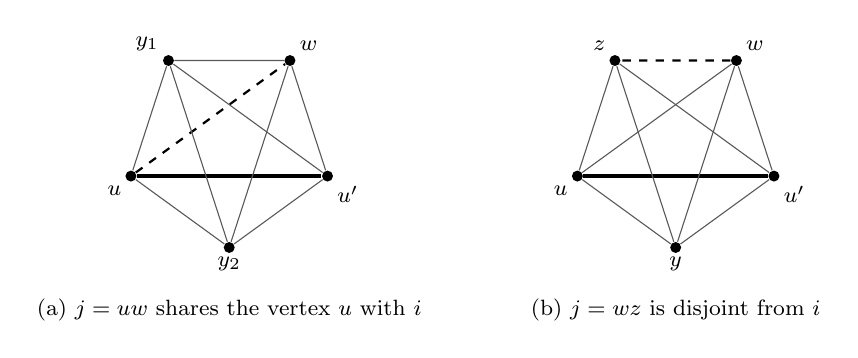
\begin{tikzpicture}[scale=1.05,
  v/.style={circle,fill=black,inner sep=1.4pt},
  lab/.style={font=\footnotesize},
  q/.style={very thick},
  j/.style={dashed,thick},
  e/.style={gray!70!black}]
  \begin{scope}
    \foreach \n/\a in {u/198,v/342,w/54,y1/126,y2/270} {\node[v] (\n) at (\a:1.25) {};}
    \node[lab,below left] at (u) {$u$}; \node[lab,below right] at (v) {$u'$};
    \node[lab,above right] at (w) {$w$}; \node[lab,above left] at (y1) {$y_1$};
    \node[lab,below] at (y2) {$y_2$};
    \draw[q] (u) -- (v);
    \draw[j] (u) -- (w);
    \foreach \a/\b in {u/y1,u/y2,v/w,v/y1,v/y2,w/y1,w/y2,y1/y2} {\draw[e] (\a) -- (\b);}
    \node[lab] at (0,-2.0) {(a) $j = uw$ shares the vertex $u$ with $i$};
  \end{scope}
  \begin{scope}[xshift=5.4cm]
    \foreach \n/\a in {u/198,v/342,w/54,z/126,y/270} {\node[v] (\n) at (\a:1.25) {};}
    \node[lab,below left] at (u) {$u$}; \node[lab,below right] at (v) {$u'$};
    \node[lab,above right] at (w) {$w$}; \node[lab,above left] at (z) {$z$};
    \node[lab,below] at (y) {$y$};
    \draw[q] (u) -- (v);
    \draw[j] (w) -- (z);
    \foreach \a/\b in {u/w,u/z,u/y,v/w,v/z,v/y,w/y,z/y} {\draw[e] (\a) -- (\b);}
    \node[lab] at (0,-2.0) {(b) $j = wz$ is disjoint from $i$};
  \end{scope}
\end{tikzpicture}

\caption{The two patterns in the proof of Lemma~\ref{lem:ext}, drawn for $k=5$. The thick edge is the queried coordinate $i=uu'$, the dashed edge the interacting coordinate $j$, and the thin edges must be present. Pattern (a) has $k-3$ further vertices, pattern (b) has $k-4$.}
\label{fig:patterns}
\end{figure}

\begin{proof}
Fix $i=uu'$. If $A_{ij}(x)=1$, then a copy of $K_k$ on a vertex set $U\ni u,u'$ contains $j$ and has all its edges except $i,j$ present. Either $j=uw$ or $j=u'w$ shares a vertex with $i$, or $j=wz$ is disjoint from $i$ (Figure~\ref{fig:patterns}). So the number of such $j$ is at most $X_u+X_{u'}+X_0$, where $X_u$ counts the sets $U$ with a distinguished vertex $w$ such that all pairs in $U$ except $uu',uw$ are present, $X_{u'}$ is symmetric, and $X_0$ counts the sets $U$ with a distinguished pair $\{w,z\}$ such that all pairs except $uu',wz$ are present.

Under $\nu$ the variables $(x_f)_{f\ne i}$ are independent Booleans, and each count is a homogeneous polynomial of degree $q:=s-2$ in them with coefficients in $\{0,1\}$, since a configuration is determined by its set of required edges (here $k\ge4$). Under $\nu$, each has expectation at most $\bar\mu:=k^2n^{k-2}p^{s-2}=k^2c_0^{s-2}n^\theta$, using $\theta(s-2)=k-2-\theta$. We use the inequality of Kim and Vu~\cite{KV00}: for a polynomial $X$ of degree at most $q$ with coefficients in $[0,1]$ in $m$ independent Boolean variables and $\lambda>1$,
\[\Pr\bigl[\abs{X-\E X}>a_q(\mathcal E_0\mathcal E_1)^{1/2}\lambda^q\bigr]\le2e^2e^{-\lambda}m^{q-1},\]
where $a_q=8^q(q!)^{1/2}$, $\partial_AX$ is the partial derivative of $X$ with respect to the variables in a set $A$, $\mathcal E_0:=\max_{\abs A\ge0}\E[\partial_AX]$ and $\mathcal E_1:=\max_{\abs A\ge1}\E[\partial_AX]$.

Let $X=X_u$ or $X_0$ and let $A$ be a nonempty set of variables with $\partial_AX\ne0$. Every required edge has an endpoint outside $\{u,u'\}$. Let $\Sigma$ be the set of these endpoints of the edges of $A$, and fix the roles that the vertices of $\Sigma$ play in the pattern, at a cost of a factor $k^k$. Let $e(\Sigma)$ be the number of required edges inside $\Sigma\cup\{u,u'\}$, so $\abs A\le e(\Sigma)$. A configuration counted by $\partial_AX$ is determined by its other $k-2-\abs\Sigma$ vertices, and it needs its other $s-2-\abs A\ge s-2-e(\Sigma)$ edges. Hence $\E[\partial_AX]\le k^kn^{k-2-\abs\Sigma}p^{s-2-e(\Sigma)}=k^{k-2}\bar\mu/\lambda_\Sigma$ with $\lambda_\Sigma:=n^{\abs\Sigma}p^{e(\Sigma)}$. We claim that
\begin{equation}\label{eq:sub}
\lambda_\Sigma\ge c_0^s\,n^{1/(k+1)}\qquad\text{for every nonempty }\Sigma.
\end{equation}
For $X_u$, let $\Sigma$ contain $a$ of the vertices other than $u,u',w$, and $\epsilon\in\{0,1\}$ copies of $w$. Then $e(\Sigma)=2a+\binom a2+\epsilon(1+a)$, and $\log_n(\lambda_\Sigma/c_0^{e(\Sigma)})$ equals $a(k-2-a)/(k+1)$ for $\epsilon=0$ and $1\le a\le k-3$, and $(-a^2+a(k-4)+k-1)/(k+1)$ for $\epsilon=1$ and $0\le a\le k-3$. The first is at least $(k-3)/(k+1)$. The second is concave in $a$, with values $(k-1)/(k+1)$ at $a=0$ and $2/(k+1)$ at $a=k-3$. For $X_0$, with $a$ vertices other than $u,u',w,z$ and $\epsilon\in\{0,1,2\}$ of $w,z$, $e(\Sigma)=2a+\binom a2+\epsilon(2+a)$. The exponents are $a(k-2-a)/(k+1)$, $(-a^2+a(k-4)+k-3)/(k+1)$ and $(-a^2+a(k-6)+2k-6)/(k+1)$, which are at least $(k-3)/(k+1)$, $(k-3)/(k+1)$ and $2/(k+1)$ for $0\le a\le k-4$ (and $a\ge1$ when $\epsilon=0$). All are at least $1/(k+1)$, and $c_0^{e(\Sigma)}\ge c_0^s$, which proves~\eqref{eq:sub}.

So $\mathcal E_1\le k^{k-2}c_0^{-s}n^{-1/(k+1)}\bar\mu$, and $\mathcal E_0\le\bar\mu$ for $n\ge n_0(k,c_0)$. With $\lambda:=n^{1/(2(k+1)q)}/C_3$ for a suitable $C_3=C_3(k,c_0)$, $a_q(\mathcal E_0\mathcal E_1)^{1/2}\lambda^q\le\bar\mu$, so $X\le2\bar\mu$ outside probability $2e^2e^{-\lambda}m^{q-1}$, where $m\le sn^2$; here $\lambda>1$ for large $n$. A union bound over the $sn^2$ edges $i$ and the three counts, and Lemma~\ref{lem:mono} (the bad event is increasing), prove the lemma with $C_2=6k^2$ and any $\delta<1/(2(k+1)q)$, for large $n$.
\end{proof}

\begin{proof}[Proof of Theorem~\ref{thm:clique}]
We verify the hypotheses of Proposition~\ref{prop:master}. Let $d_0:=\lceil8\Delta p\rceil\le9\Delta p$, and let $b$ be $\exp(-n^\delta)$ plus the probability $2kn\exp(-c\Delta p)$ that the maximum degree exceeds $d_0$.

(P). A copy $T'\ne T$ created by adding $T$ shares $a$ vertices with $T$ for some $2\le a\le k-1$ and needs its $s-\binom a2$ edges outside $T$ to be present. There are at most $\binom kan^{k-a}$ such copies. Since $s-\binom a2=(k-a)(k+a-1)/2$, the expected number is at most $\binom kac_0^{s-\binom a2}n^{(k-a)(2-a)/(k+1)}\le\binom kac_0^{s-\binom a2}$, and Lemma~\ref{lem:mono} gives $\mu^-(\Ev_T)\ge1/2$ for small $c_0$.

(S). Fix the edges outside $\st(w)$. A copy of $K_k$ through $w$ consists of star edges $wa_1,\dots,wa_{k-1}$ and a $K_{k-1}$ on $a_1,\dots,a_{k-1}$. If $A_{wa,wa'}(x)=1$, then $aa'$ is a present edge outside the star. So $N_{wa,\st(w)}(x)$ is at most the degree of $a$ outside the star. On the event $\Ev_w$ that the outside graph has maximum degree at most $d_0$, (S) holds with $d_s:=d_0\le9(k-1)np$. Then
\[\frac{pd_s}R\le\frac{9(k-1)np^2}{(np)^{2/3}}=9(k-1)c_0^{4/3}n^{\frac13-\frac43\theta}=9(k-1)c_0^{4/3}n^{\frac{k-7}{3(k+1)}}\le9(k-1),\]
so $S\le2+81(k-1)^2$ for $k\le7$.

(I) holds with $d_m:=C_2c_0^{s-2}n^\theta$ by Lemma~\ref{lem:ext}, and $pd_m=C_2c_0^{s-1}\le1/5$ for small $c_0$.

Proposition~\ref{prop:master} gives $\sqrt\sigma\le c(t+s)n^{-7/6}p^{-1/6}$ for large $n$, and $n^{7/6}p^{1/6}=c_0^{1/6}n^{7/6-1/(3(k+1))}$. As before, take $n=\lfloor N/k\rfloor$ and use~\cite[Lemma~23]{CGP26} for detection.
\end{proof}

\begin{proof}[Proof of Corollary~\ref{cor:chromatic}]
By~\cite[Theorem~1.3(i)]{GZ26}, $Q(\Sub_H)=\Omega(Q(\Sub_{K_r}))$ with $r=\min\{\chi,6\}$, and the same holds for finding. Apply Theorem~\ref{thm:clique} with $r=4,5,6$.
\end{proof}

\section{Denser patterns: extension counts}\label{sec:ext}

The degree bounds of Section~\ref{sec:2conn} count the extensions of a spanning tree, and they hold up to $p\approx n^{-(v-2)/(v-1)}$. For denser $H$ more edges of a copy must be present, and counting the extensions of a larger pattern allows larger densities. This section turns this into a general criterion and applies it to complete bipartite graphs.

\paragraph{Rooted patterns.} A \emph{rooted pattern} in $H$ is a triple $(S,Q,F)$ with $Q\subseteq S\subseteq V(H)$ and $F\subseteq E(H[S])$ such that no edge of $F$ lies inside $Q$. For $0<\theta<1$ put
\[\varepsilon_\theta(S,Q,F):=\max_{Q\subseteq U\subseteq S}\bigl(\abs{S\setminus U}-\theta\abs{F\setminus F[U]}\bigr)\ge0,\]
where $F[U]$ is the set of edges of $F$ inside $U$; the term $U=S$ is $0$. The pattern is \emph{safe at $\theta$} if $\abs{U\setminus Q}-\theta\abs{F[U]}>0$ for every $U$ with $Q\subsetneq U\subseteq S$. For an injective map $\rho$ from $Q$ to $V(G)$ and a set $Z\subseteq V(G)$, let $X_\rho(x)$ be the number of injective maps $\psi:S\to V(G)\setminus Z$ that extend $\rho$ and map every edge of $F$ to an edge of $G$ present in $x$.

\begin{lemma}\label{lem:count}
Let $(S,Q,F)$ be a rooted pattern in which every vertex of $S\setminus Q$ lies on an edge of $F$, let $0<\theta<1$, $p=c_0n^{-\theta}$ with $c_0\le1$, and $\varepsilon:=\varepsilon_\theta(S,Q,F)$. There is $C$ depending only on $H$, not on $c_0$, such that for $n\ge n_0(H)$, every $\rho$ and $Z$,
\[\nu\bigl[X_\rho>Cn^\varepsilon(\log n)^{\abs F}\bigr]\le n^{-20}.\]
If the pattern is safe at $\theta$, then there is $\delta>0$ such that $\nu[X_\rho>C\bar\mu]\le\exp(-n^\delta)$ for $n\ge n_0(H,c_0)$, with the same $C$, where $\bar\mu:=(vn)^{\abs{S\setminus Q}}p^{\abs F}$.
\end{lemma}

\begin{proof}
Put $q:=\abs F$; if $q=0$ then $S=Q$ and $X_\rho\le1$. Each $\psi$ contributes the monomial $\prod_{f\in F}x_{\psi(f)}$, of degree $q$ since $\psi$ is injective. The monomial determines the image of $S\setminus Q$, because every vertex of $S\setminus Q$ lies on an edge of $F$, so at most $v!$ maps $\psi$ give the same monomial. Hence $X_\rho/v!$ is a homogeneous polynomial of degree $q$ with coefficients in $[0,1]$ in the independent Boolean variables $x_g$, $g\in J$. Let $A$ be a set of variables with $\partial_AX_\rho\ne0$, and let $U\supseteq Q$ consist of $Q$ and the vertices of $S$ that $\psi$ maps to endpoints of edges of $A$, for some $\psi$ counted by $\partial_AX_\rho$. Then $\abs A\le\abs{F[U]}$. There are at most $2^v$ choices of $U$ and at most $(2e_H+v)^v$ of $\psi|_U$, whose values are endpoints of edges of $A$ or values of $\rho$; the other vertices have at most $vn$ images each, and the other $q-\abs A\ge q-\abs{F[U]}$ edges must be present. So
\[\E[\partial_AX_\rho]\le v!\,2^v(2e_H+v)^v\max_{Q\subseteq U\subseteq S}(vn)^{\abs{S\setminus U}}p^{q-\abs{F[U]}}\le C'n^\varepsilon,\]
including $A=\emptyset$. The inequality of Kim and Vu, quoted in the proof of Lemma~\ref{lem:ext}, with $\lambda:=22q\log n$ gives $X_\rho\le C'n^\varepsilon+v!\,a_qC'n^\varepsilon\lambda^q$ outside probability $2e^2e^{-\lambda}(e_Hn^2)^{q-1}\le n^{-20}$ for large $n$.

If the pattern is safe, let $\delta_0>0$ be the minimum of $\abs{U\setminus Q}-\theta\abs{F[U]}$ over $U\ne Q$. The term for $U\ne Q$ above equals $v^{\abs{S\setminus U}}\bar\mu\,v^{-\abs{S\setminus Q}}c_0^{-\abs{F[U]}}n^{-(\abs{U\setminus Q}-\theta\abs{F[U]})}$, so $\mathcal E_1\le C''c_0^{-q}n^{-\delta_0}\bar\mu$ and $\mathcal E_0\le C''\bar\mu$ for large $n$. With $\lambda:=n^{\delta_0/(2q)}/C_3$ as in the proof of Lemma~\ref{lem:ext}, the deviation is at most $C''\bar\mu$ outside probability $\exp(-n^{\delta})$ for every $\delta<\delta_0/(2q)$ and large $n$. Since $p\le n^{-\theta}$, the constants $C'$ and $C''$ depend only on $H$.
\end{proof}

Let $e_{\max}(j)$ be the largest number of edges of $H$ spanned by $j$ vertices, and
\[\theta_P(H):=\max_{2\le j\le v-1}\frac{v-j}{e_H-e_{\max}(j)}.\]
We call $\theta$ \emph{star-admissible} if for every vertex $x_0$ of $H$ and all distinct neighbours $y,z$ of $x_0$ there is a set $S\subseteq V(H)\setminus\{x_0\}$ containing $y$ and $z$ such that the pattern $(S,\{y\},E(H[S]))$ satisfies $\varepsilon_\theta<2/3+\theta/3$, or $\varepsilon_\theta=2/3+\theta/3$ and is safe at $\theta$.

\begin{theorem}\label{thm:ext}
Let $H$ be a fixed connected graph on $v\ge3$ vertices and let $\theta_P(H)\le\theta<1$ be star-admissible. If $\theta=\theta_P(H)$, assume in addition that $(V(H),i,E(H)\setminus\{i,j\})$ is safe at $\theta$ for all distinct edges $i,j$ of $H$. Then detecting or finding $H$ takes $\Omega(N^{7/6-\theta/6})$ quantum queries.
\end{theorem}

\begin{proof}
Let $p:=c_0n^{-\theta}$ and verify the hypotheses of Proposition~\ref{prop:master}; then $R=(np)^{2/3}\ge1$ for large $n$. Let $\eta:=n^{-15}$ be the failure probability $b$ of Proposition~\ref{prop:master}.

(P). A copy $T'\ne T$ created by adding $T$ shares $j\ge2$ vertices with $T$. For $j\le v-1$ there are at most $\binom vjC_Hn^{v-j}$ such copies, each needing at least $e_H-e_{\max}(j)$ present edges outside $T$, so the expected number is at most $\binom vjC_Hc_0n^{(v-j)-\theta(e_H-e_{\max}(j))}\le\binom vjC_Hc_0$. For $j=v$ the expected number is $O(p)$. Lemma~\ref{lem:mono} gives $\mu^-(\Ev_T)\ge1/2$ for small $c_0$.

(S). Fix $w$. Suppose $A_{wu,wu'}(x)=1$ through a copy $\varphi(H)$ with $\varphi(x_0)=w$, $\varphi(y)=u$, $\varphi(z)=u'$, and let $S$ be the set chosen for $(x_0,y,z)$. If some vertex of $S\setminus\{y\}$ lies on no edge of $H[S]$, then the term for $U=S$ minus that vertex gives $\varepsilon_\theta\ge1>2/3+\theta/3$, so this does not happen. The edges of $H[S]$ avoid $x_0$, so $\varphi$ maps them outside $\st(w)$, where they are present. Hence $\varphi|_S$ is counted by $X_\rho$ with $\rho(y)=u$ and $Z=\{w\}$, and $u'=\varphi(z)$. So $N_{wu,\st(w)}(x)$ is at most the sum of these counts over the at most $v^3$ triples $(x_0,y,z)$. They depend only on the edges outside $\st(w)$, and the event that one of them exceeds the bound of Lemma~\ref{lem:count} is increasing. By Lemma~\ref{lem:count}, the union bound over $u$ and Lemma~\ref{lem:mono}, (S) holds with failure probability at most $\eta$ and either $d_s:=Cv^3n^\varepsilon(\log n)^{e_H}$ with $\varepsilon<2/3+\theta/3$, or $d_s:=Cv^3\bar\mu$ with $\bar\mu\le c\,c_0^{\abs F}n^{2/3+\theta/3}$. In the first case $pd_s/R=c_0^{1/3}n^{\varepsilon-2/3-\theta/3}Cv^3(\log n)^{e_H}\to0$; in the second $pd_s/R\le cc_0^{1/3}$. (Different triples may use different cases; the bounds add.) So $pd_s\le R$ for small $c_0$ and large $n$.

(I). Suppose $A_{ij}(x)=1$ through a copy $\varphi(H)$, and let $i_H,j_H$ be the edges of $H$ mapped to $i$ and $j$. Then $\varphi$ is counted by $X_\rho$ for the pattern $P_{i_H,j_H}:=(V(H),i_H,E(H)\setminus\{i_H,j_H\})$ with $\rho=\varphi|_{i_H}$ and $Z=\emptyset$, and $j=\varphi(j_H)$. Since $\theta_P\le\theta<1$, $H$ has minimum degree at least $2$: a vertex of degree one gives the ratio $1$ for $a=v-1$. So every vertex outside $i_H$ lies on an edge of this pattern. For $\overline U:=V(H)\setminus U$, the number of edges of $P_{i_H,j_H}$ that meet $\overline U$ is at least $e'-1$, where $e'$ is the number of edges of $H$ that meet $\overline U$. Since $U$ contains $i_H$, it has at least two vertices and $e_H-e'\le e_{\max}(v-\abs{\overline U})$, so $\abs{\overline U}\le\theta_Pe'\le\theta e'$ for $\overline U\ne\emptyset$. Hence each term of $\varepsilon_\theta(P_{i_H,j_H})$ is at most $\abs{\overline U}-\theta(e'-1)\le\theta$, with strict inequality when $\theta>\theta_P$. If $\theta>\theta_P$, Lemma~\ref{lem:count} gives $d_m:=Ce_H^2n^\varepsilon(\log n)^{e_H}$ with $\varepsilon<\theta$, so $pd_m\to0$. If $\theta=\theta_P$, safety gives $d_m:=Ce_H^2\bar\mu$ with $p\bar\mu=c\,c_0^{e_H-1}n^{(v-2)-\theta(e_H-1)}\le cc_0^{e_H-1}$, since the term for $U=i_H$ is at most $\theta$. So $pd_m\le1/5$ for small $c_0$. The failure probability is at most $\eta$ by Lemma~\ref{lem:mono}.

Proposition~\ref{prop:master} gives $\sqrt\sigma\le c(t+e_H)n^{-7/6}p^{-1/6}$ for large $n$, since $n^4\eta\le n^{-11}$. Take $n=\lfloor N/v\rfloor$ and use~\cite[Lemma~23]{CGP26} for detection.
\end{proof}

\begin{corollary}\label{cor:kab}
Let $3\le a\le b$ and $\theta_{a,b}:=(3a+3b-8)/(3(a-1)b+1)$. Detecting or finding $K_{a,b}$ takes $\Omega(N^{7/6-\theta_{a,b}/6})$ quantum queries. Detecting or finding $K_{2,3}$ takes $\Omega(N^{16/15})$, and $K_{2,b}$ with $b\ge4$ takes $\Omega(N^{15/14})$.
\end{corollary}

For $K_{r,r}$ with $r\ge3$ the exponent is $7/6-(3r-4)/(3(3r^2-3r+1))$: $41/38$ for $r=3$, $81/74$ for $r=4$ and $615/542\approx1.135$ for $r=10$, where Theorem~\ref{thm:2conn} gives $115/114$ and~\cite{GZ26} gives $181/180$. A comparison with exact fractions shows that it exceeds $\beta_r$ of~\cite[(68)]{GZ26} exactly for $r\le18$ among $10\le r\le20$; since $\beta_r$ increases and the exponent here stays below $7/6$, while $\beta_{20}>7/6$, the bounds of~\cite{GZ26} are larger for all $r\ge19$.

\begin{proof}
Let $H=K_{a,b}$ with sides $A$ and $B$, $\abs A=a\le b=\abs B$. A copy sharing $a_1\ge1$ vertices of $A$ and $b_1\ge1$ of $B$ with $T$, $(a_1,b_1)\ne(a,b)$, gives the ratio $(a+b-a_1-b_1)/(ab-a_1b_1)$. With $\bar a=a-a_1$ and $\bar b=b-b_1$, the quantity $(a+b-2)(\bar ab+\bar ba-\bar a\bar b)-(ab-1)(\bar a+\bar b)$ is bilinear in $(\bar a,\bar b)$, with values $0$, $(a-1)(b-1)^2$, $(b-1)(a-1)^2$ and $0$ at the corners of $[0,a-1]\times[0,b-1]$, so it is nonnegative and $\theta_P=(a+b-2)/(ab-1)$; shared sets with $a_1=0$ or $b_1=0$ contain no edge of $T$ and cannot create a copy.

Let $a\ge3$ and $\theta=\theta_{a,b}$. First, $\theta>\theta_P$, since
\[(3a+3b-8)(ab-1)-(a+b-2)(3ab-3b+1)=3b^2+ab-4a-10b+10>0\]
for $3\le a\le b$. Also $\theta<1$, since $3(a-1)b+1-(3a+3b-8)=3((a-2)(b-1)+1)>0$, and $\theta(a-1)\ge1$, which is equivalent to $(3a-8)(a-1)\ge1$. For star-admissibility take $S=V(H)\setminus\{x_0\}$. If $x_0\in A$, then $y,z\in B$, and the set $\overline U=S\setminus U$ with $\alpha$ vertices in $A$ and $\beta$ in $B$ meets $\alpha b+\beta(a-1)-\alpha\beta$ edges of $H-x_0$. The term $\abs{\overline U}-\theta(\alpha b+\beta(a-1)-\alpha\beta)$ is bilinear in $(\alpha,\beta)\in[0,a-1]\times[0,b-1]$, so its maximum is at a corner. The corner values are $0$, $(a-1)(1-\theta b)\le0$, $(b-1)(1-\theta(a-1))\le0$ and $a+b-2-\theta(a-1)b=2/3+\theta/3$, by the definition of $\theta$. So $\varepsilon_\theta=2/3+\theta/3$. The pattern is safe: for $U\ne\{y\}$ with $\alpha'$ vertices of $A$ and $\beta'$ vertices of $B\setminus\{y\}$, $\abs{U\setminus\{y\}}-\theta\abs{F[U]}=\alpha'+\beta'-\theta\alpha'(\beta'+1)$. For $\alpha'=0$ this is $\beta'>0$. For $\alpha'\ge1$ it is linear in $\beta'$, with value $\alpha'(1-\theta)>0$ at $\beta'=0$ and $\alpha'(1-\theta b)+b-1$ at $\beta'=b-1$, which is linear in $\alpha'$ with values $b(1-\theta)>0$ and $2/3+\theta/3>0$ at $\alpha'=1$ and $\alpha'=a-1$. If $x_0\in B$, the same computation with $\alpha\le a-1$ vertices in $A$ and $\beta\le b-1$ in $B$ gives the corners $0$, $(a-1)(1-\theta(b-1))\le0$, $(b-1)(1-\theta a)\le0$ and $a+b-2-\theta a(b-1)\le a+b-2-\theta(a-1)b$; if $a<b$ the last is strictly smaller, and if $a=b$ the case is symmetric to $x_0\in A$. Theorem~\ref{thm:ext} applies.

Let $a=2$, and let $x_0$, $y$, $z$ be as in the definition, so $y,z$ lie on the side not containing $x_0$. Take $S=\{y,l,z\}$ with $l\ne x_0$ on the side of $x_0$, so that $H[S]$ is the path $y\,l\,z$. The terms of $\varepsilon_\theta$ are $2-2\theta$, $1-\theta$, $1-2\theta$ and $0$ for $U=\{y\}$, $\{y,l\}$, $\{y,z\}$, $S$, so $\varepsilon_\theta=2-2\theta\le2/3+\theta/3$ if and only if $\theta\ge4/7$, and the path is safe since $1-\theta$, $1$ and $2-2\theta$ are positive. Here $\theta_P=b/(2b-1)$, which is $3/5$ for $b=3$, $4/7$ for $b=4$ and smaller for $b\ge5$. So $\theta=\max\{4/7,b/(2b-1)\}$ is star-admissible. If $b\in\{3,4\}$, then $\theta=\theta_P$, and the patterns $P_{i,j}$ are safe: with $i=uu'$, $u\in A$, a set $U\setminus i$ with $\alpha\in\{0,1\}$ vertices of $A$ and $\beta$ vertices of $B$ spans at most $\beta+\alpha(1+\beta)$ edges of $P_{i,j}$, and at most $2b-2$ if $U=V(H)$. For $\alpha=0$ the safety term is $\beta(1-\theta)>0$; for $\alpha=1$ and $\beta\le b-2$ it is at least $1+\beta-\theta(1+2\beta)>0$, since $(1+\beta)/(1+2\beta)\ge(b-1)/(2b-3)>b/(2b-1)$; and for $U=V(H)$ it is $b-\theta(2b-2)>0$. Theorem~\ref{thm:ext} gives the exponents $7/6-1/10=16/15$ and $7/6-2/21=15/14$.
\end{proof}

\begin{remark}\label{rem:octa}
The octahedron $K_{2,2,2}$ has chromatic number $3$, so the best previous bound known to us is $N^{13/12}$~\cite{CGZ26}. Here $\theta_P=4/11$. For a vertex $x_0$ and adjacent neighbours $y,z$, the pattern $S=\{y,z\}$ has $\varepsilon_\theta=1-\theta$. For the non-adjacent pairs, $S=V(H)\setminus\{x_0\}$ induces a wheel on five vertices with hub the antipode of $x_0$, and $\varepsilon_\theta=4-8\theta$ for $\theta\le1/2$, which equals $2/3+\theta/3$ at $\theta=2/5$; this pattern is safe at $2/5$. Theorem~\ref{thm:ext} gives $\Omega(N^{11/10})$.
\end{remark}

The conditions of Theorem~\ref{thm:ext} are finite and can be checked by a computer. A script computes the smallest $\theta\ge\theta_P$ that is star-admissible and, for $\theta>\theta_P$ automatically and for $\theta=\theta_P$ through the safety of $P_{i,j}$, satisfies (I), minimizing over all sets $S$ for each triple $(x_0,y,z)$; it also checks that each condition that is tight at this $\theta$ has a safe pattern. It reproduces Theorems~\ref{thm:2conn} and~\ref{thm:clique} for $C_3$, $C_4$, $K_4$ and $K_5$, and it gives the value $\theta_{a,b}$ of Corollary~\ref{cor:kab} (and $\max\{4/7,b/(2b-1)\}$ for $a=2$) by brute force for $a+b\le8$ and by a computation over vertex types for all $2\le a\le b\le30$. The scripts are in \url{https://github.com/ssenge/LAIF}, in the folders \texttt{complete-bipartite-quantum-lower-bounds} and \texttt{two-connected-subgraph-quantum-lower-bounds}.

\section{Limits of the method}\label{sec:limits}

\begin{figure}[t]
\centering
% Lower bound exponents for K_k detection: previous best and this work.
% Previous: k = 3 from [CGZ26], k >= 4 the larger of [GZ26] and the bound for K_{k-1}.
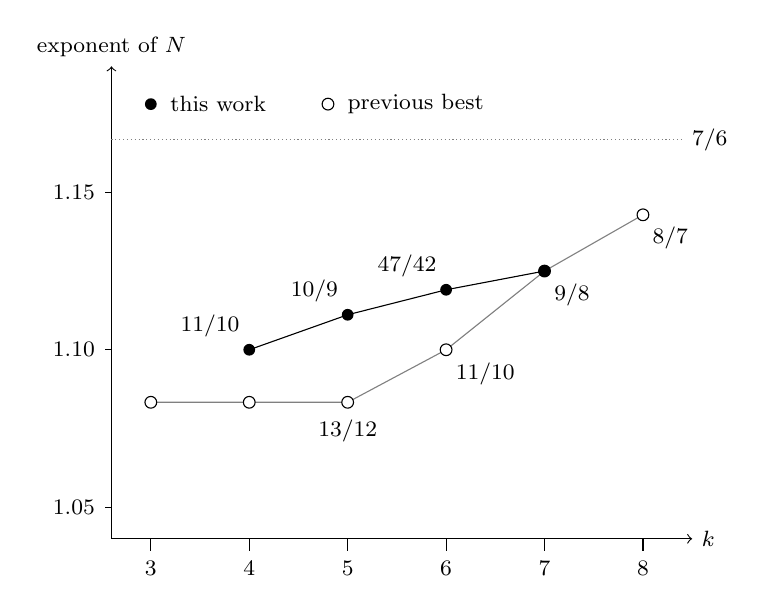
\begin{tikzpicture}[x=1.25cm,y=40cm,
  lab/.style={font=\footnotesize},
  old/.style={circle,draw,fill=white,inner sep=1.5pt},
  new/.style={circle,fill=black,inner sep=1.5pt}]
  \draw[->] (2.6,1.04) -- (8.5,1.04) node[lab,right] {$k$};
  \draw[->] (2.6,1.04) -- (2.6,1.19) node[lab,above] {exponent of $N$};
  \foreach \k in {3,...,8} {\draw (\k,1.04) -- (\k,1.036) node[lab,below] {\k};}
  \foreach \y/\t in {1.05/1.05,1.10/1.10,1.15/1.15} {\draw (2.6,\y) -- (2.53,\y) node[lab,left] {\t};}
  \draw[densely dotted,gray] (2.6,1.16667) -- (8.4,1.16667) node[lab,right,black] {$7/6$};
  % previous best: 13/12, 13/12, 13/12, 11/10, 9/8, 8/7
  \draw[gray] (3,1.08333) -- (4,1.08333) -- (5,1.08333) -- (6,1.1) -- (7,1.125) -- (8,1.14286);
  \foreach \k/\y in {3/1.08333,4/1.08333,5/1.08333,6/1.1,7/1.125,8/1.14286} {\node[old] at (\k,\y) {};}
  % this work: 11/10, 10/9, 47/42, 9/8
  \draw (4,1.1) -- (5,1.11111) -- (6,1.11905) -- (7,1.125);
  \foreach \k/\y in {4/1.1,5/1.11111,6/1.11905,7/1.125} {\node[new] at (\k,\y) {};}
  \node[lab,anchor=south east] at (4,1.101) {$11/10$};
  \node[lab,anchor=south east] at (5,1.112) {$10/9$};
  \node[lab,anchor=south east] at (6,1.120) {$47/42$};
  \node[lab,anchor=north] at (5,1.081) {$13/12$};
  \node[lab,anchor=north west] at (6,1.099) {$11/10$};
  \node[lab,anchor=north west] at (7,1.124) {$9/8$};
  \node[lab,anchor=north west] at (8,1.142) {$8/7$};
  % legend
  \node[new] at (3.0,1.178) {}; \node[lab,anchor=west] at (3.1,1.178) {this work};
  \node[old] at (4.8,1.178) {}; \node[lab,anchor=west] at (4.9,1.178) {previous best};
\end{tikzpicture}

\caption{Lower bound exponents for $K_k$ detection. Open circles: the previous best, from~\cite{CGZ26} for $k\le5$ and from the clique collision bound of~\cite[Corollary~4.6]{GZ26} for $k\ge6$, which is $1/2+\ell(2k-\ell-1)/(2(k-1)(\ell+1))$ maximized over $\ell$, minus $o(1)$. Filled circles: Theorem~\ref{thm:clique}.}
\label{fig:exponents}
\end{figure}

Whenever its hypotheses hold with bounded $pd_s/R$, Proposition~\ref{prop:master} gives $t=\Omega(n^{7/6}p^{1/6})$, so the bound is limited by the largest density at which (P), (S) and (I) hold.

\paragraph{Cut vertices.} Proposition~\ref{prop:master} with the degree bounds of Section~\ref{sec:2conn} does not apply directly when a cut vertex $w$ of $H$ joins two blocks with cycles. In the star of a vertex playing the role of $w$, an edge $wa$ in one block interacts with every edge $wa'$ in the other block for which $a'$ lies in a present copy of that block minus its edges at $w$. When this graph is a tree, as for two four-cycles sharing a vertex, the number of such $a'$ is of order $n(np)^{\beta-2}$ for a block with $\beta$ vertices, so $pd_s\approx(np)^{\beta-1}$ exceeds $R$ at every density with $np\to\infty$. Lemma~\ref{lem:blockred} avoids the problem by reducing to a single block. For denser blocks Theorem~\ref{thm:ext} applies directly, since a dense pattern on the far side of the cut vertex has few extensions. For two copies of $K_{3,3}$ sharing a vertex, $\theta_P=5/9$ and $\theta=13/19$ is star-admissible, with the pattern $K_{3,3}$ minus the cut vertex on the far side, which gives $\Omega(N^{20/19})$. Lemma~\ref{lem:blockred} transfers every lower bound for $B$ to $H$, so with Corollary~\ref{cor:kab} it gives more here: $\Omega(N^{41/38})$, by (a).

\paragraph{Densities.} The planting condition alone allows $p\approx n^{-\theta_P}$, with $\theta_P$ as in Section~\ref{sec:ext}. For cycles $\theta_P=(v-2)/(v-1)$, so for them hypothesis (P) allows no larger density. For $K_k$ with $k\le7$ and for $K_{2,3}$ and $K_{2,4}$ the bounds reach $\theta_P$. For $K_{r,r}$ with $r\ge3$ star-admissibility, minimized over all sets $S$, is the binding condition, and for $K_k$ with $k\ge8$ it caps the density at $n^{-1/4}$, which gives only $N^{9/8}$. The exponent $7/6-\theta/6$ stays below $7/6$ for every $H$, so for large $r$ the random constructions of~\cite{GZ26} give more for $K_{r,r}$.

\paragraph{Large cliques.} For $k\ge8$, the planting condition allows $p$ above $n^{-1/4}$, but there $pd_s\approx np^2$ exceeds $R=(np)^{2/3}$, and $S\approx n^2p^4/R^2$. The resulting heuristic error bound is of order $n^{-3}(R/p+n^2p^3/R+n^2p/R^2)$. For $p\ge n^{-1/4}$ it is smallest at $R=np^2$, where it is of order $p/n^2$, which gives $t\gtrsim np^{-1/2}$, decreasing in $p$. So the best choice is $p\approx n^{-1/4}$, giving $N^{9/8}$, below the bound $N^{8/7-o(1)}$ of~\cite{GZ26} for $K_8$ (Figure~\ref{fig:exponents}). Lemma~\ref{lem:sumproj} may be lossy here, so this is a limit of the present analysis rather than of conditioned random graphs.

\paragraph{Tightness.} For triangles, the bound $n^{7/6}p^{1/6}$ gives lower bounds for sparse graphs that are tight up to polylogarithmic factors in a range of edge counts~\cite{CGZ26}. We do not know whether $n^{7/6}p^{1/6}$ is tight on our hard inputs for any other pattern.

\section*{Use of AI}

Claude Opus 5.5 (Anthropic) was used throughout this research: to explore approaches, to develop and check proofs, to write the check scripts, and to draft the text.

\begin{thebibliography}{99}\small

\bibitem{Bel26} A.~Belovs. Tight quantum lower bound for $k$-distinctness. FOCS 2026, to appear. arXiv:2604.05133.

\bibitem{BR12} A.~Belovs, B.~W.~Reichardt. Span programs and quantum algorithms for st-connectivity and claw detection. ESA 2012, LNCS 7501, 193--204.

\bibitem{CK11} A.~M.~Childs, R.~Kothari. Quantum query complexity of minor-closed graph properties. STACS 2011, LIPIcs 9, 661--672.

\bibitem{CGP26} A.~Cornelissen, A.~S.~Gilani, S.~Patro. Quantum algorithms for path and cycle containment problems. APPROX/RANDOM 2026, LIPIcs 392, 72:1--72:23. arXiv:2605.09017.

\bibitem{CGZ26} A.~Cornelissen, A.~S.~Gilani, X.~Zhou. A quantum lower bound for triangle finding. arXiv:2611.06751v1, 2026.

\bibitem{GZ26} A.~S.~Gilani, X.~Zhou. Superlinear quantum query lower bounds for subgraph detection. arXiv:2609.40263, 2026.

\bibitem{KV00} J.~H.~Kim, V.~H.~Vu. Concentration of multivariate polynomials and its applications. \emph{Combinatorica} 20(3):417--434, 2000.

\bibitem{LMS12} T.~Lee, F.~Magniez, M.~Santha. Learning graph based quantum query algorithms for finding constant-size subgraphs. \emph{Chicago Journal of Theoretical Computer Science} 2012(10):1--21, 2012.

\bibitem{SS06} R.~\v{S}palek, M.~Szegedy. All quantum adversary methods are equivalent. \emph{Theory of Computing} 2(1):1--18, 2006.

\bibitem{Zha04} S.~Zhang. On the power of Ambainis's lower bounds. ICALP 2004, LNCS 3142, 1238--1250.

\bibitem{Zhu12} Y.~Zhu. Quantum query complexity of constant-sized subgraph containment. \emph{International Journal of Quantum Information} 10(3):1250019, 2012.

\end{thebibliography}

\end{document}
